\hyperdef{recursive}{data}{\chapter{Recursive Data Types}}
%\coursecopyright

\emph{Recursive data types} play a central role in programming.  From a
Mathematical point of view, recursive data types are what induction is
about.  Recursive data types are specified by \emph{recursive definitions}
that say how to build something from its parts.  These definitions have
two parts:
\begin{itemize}
\item \textbf{Base case(s)} that don't depend on anything else.
\item \textbf{Constructor case(s)} that depend on previous cases.
\end{itemize}

\hyperdef{paren}{string}{\subsection{Strings of Parentheses}}

Let $\prns$ be the set of all strings of parentheses.  For example,
the following two strings are in $\prns$:
\begin{equation}\label{2strings}
\mtt{())((((())}\quad \text{and}\quad \mtt{((())())()}
\end{equation}
Since we're just starting to study recursive data, just for practice we'll
formulate $\prns$ as a recursive data type,

\begin{definition}\label{prns-def}
The data type, $\prns$, of strings of parentheses is defined recursively:

\begin{itemize}

\item \textbf{Base case:} The \term{empty string}, $\emptystring$, is in
  $\prns$.

\item \textbf{Constructor case:} If $s \in \prns$, then
$s\mtt{)}$ and $s\mtt{(}$ are in $\prns$.

\end{itemize}

\end{definition}

Here we're writing $s\mtt{)}$ to indicate the string that is sequence of
parentheses (if any) in the string $s$, followed by a right parenthesis;
similarly for $s\mtt{(}$.

A string, $s \in \prns$, a called a \term{matched string} if its
parentheses ``match up'' in the usual way.  For example, the left hand
string above is not matched because its second right parenthesis does not
have a matching left parenthesis.  The string on the right is matched.

One precise way to determine if a string is matched is to start with 0 and
read the string from left to right, adding 1 to the count for each left
parenthesis and subtracting 1 from the count for each right parenthesis.
For example, here are the counts for the two strings above
\[\begin{array}{rrrrrrrrrrrrr}
& \mtt{(} & \mtt{)} & \mtt{)} & \mtt{(} & \mtt{(} & \mtt{(} & \mtt{(} &
\mtt{(} & \mtt{)} & \mtt{)} & \mtt{)} & \mtt{)}\\
0 & 1 & 0 & -1 & 0 & 1 & 2 & 3 & 4 & 3 & 2 & 1 & 0\\
\\
\\
& \mtt{(} & \mtt{(} & \mtt{(} & \mtt{)} & \mtt{)} & \mtt{(} & \mtt{)} &
\mtt{)} & \mtt{(} & \mtt{)}\\
0 & 1 & 2 & 3 & 2 & 1 & 2 & 1 & 0 & 1 & 0
\end{array}\]
A string has a \term{good count} if its running count never goes
negative and ends with 0.  So the second string above has a good count, but
the first one does not because its count went negative at the third step.
\begin{definition}\label{gc-def}
Let
\[
\GC \eqdef \set{ s \in \prns \suchthat s\ \text{has a good count}}.
\]
\end{definition}
The matched strings can now be characterized precisely as this set of
strings with good counts.  But it turns out to be really useful to
characterize the matched strings in another way as well, namely, as a
recursive data type:

\begin{definition}\label{RM-def}
Recursively define the set, $\RM$, of strings as follows:
\begin{itemize}

\item \textbf{Base case:} $\emptystring \in\RM$.

\item \textbf{Constructor case:} If $s,t \in\RM$, then
\[
\mtt{(}s\mtt{)}t \in\RM.
\]

\end{itemize}

\end{definition}


Here we're writing $\mtt{(}s\mtt{)}t$ to indicate the string that
starts with a left parenthesis, followed by the sequence of parentheses
(if any) in the string $s$, followed by a right parenthesis, and ending
with the sequence of parentheses in the string $t$.

Using this definition, we can see that $\emptystring \in\RM$ by the Base
case, so
\[
\mtt{(}\emptystring\mtt{)}\emptystring=\mtt{()}\in\RM
\]
by the Constructor case.  So now,
\begin{align*}
\mtt{(}\emptystring\mtt{)}\mtt{()} &= \mtt{()()} \in \RM
    & \text{(letting $s = \emptystring, t = \mtt{()}$)}\\
\mtt{(())}\emptystring & = \mtt{(())} \in \RM
    & \text{(letting $s = \mtt{()}, t = \emptystring$)}\\
&\ \ \mtt{(())()} \in \RM
    & \text{(letting $s = \mtt{()}, t = \mtt{()}$)}
\end{align*}
are also strings in $\RM$ by repeated applications of the Constructor
case.

\textbf{Quickie:} Verify that $\mtt{((())())()} \in \RM$.

It may not be obvious, but $\RM = \GC$.  We'll confirm this later.

\subsection{Arithmetic Expressions}
Expression evaluation is a key feature of programming languages, and
recognition of expressions as a recursive data type is a key to
understanding how they can be processed.

To illustrate this approach we'll work with a toy example: arithmetic
expressions like $3x^2 + 2x + 1$ involving only one variable, ``$x$.''
We'll refer to the data type of such expressions as $\aexp$.  Here is its
definition:

\begin{definition}\label{A}
The set, $\aexp$, of \emph{Arithmetic expressions} in the variable, $x$,
is defined recursively as follows:

\begin{itemize}
\item \textbf{Base cases:}

\begin{enumerate}

\item The variable, $x$, is in $\aexp$.

\item The arabic numeral, $\mtt{k}$, for any nonnegative integer, $k$, is
  in $\aexp$.

\end{enumerate}

\item \textbf{Constructor cases:} If $e,f \in \aexp$, then
\begin{enumerate}
\setcounter{enumi}{2}

\item $(e \sumsym f) \in \aexp$.  The expression $(e \sumsym f)$ is called a
  \term{sum}.  The \aexp's $e$ and $f$ are called the \term{components} of
  the sum; they're also called the \term{summands}.

\item $(e \prodsym f) \in \aexp$.  The expression $(e \prodsym f)$ is called a
  \term{product}.  The \aexp's $e$ and $f$ are called the
  \term{components} of the product; they're also called the
  \term{multiplier} and \term{multiplicand}.

\item $\minussym(e) \in \aexp$.  The expression $\minussym(e)$ is called a
  \term{negative}.
\end{enumerate}
\end{itemize}
\end{definition}

Notice that \aexp's are fully parenthesized, and exponents aren't allowed.
So the $\aexp$ version of the polynomial expression $3x^2 + 2x + 1$ would
officially be written as
\begin{equation}\label{fullparens}
((\mtt{3} \prodsym (x \prodsym x)) \sumsym ((\mtt{2} \prodsym x) \sumsym \mtt{1})).
\end{equation}
These parentheses and $\ast$'s clutter up examples, so we'll often use
simpler expressions like ``$3x^2 + 2x + 1$'' instead
of~\eqref{fullparens}.  But it's important to recognize that $3x^2 + 2x +
1$ is not an \aexp; it's an \emph{abbreviation} for an $\aexp$.

\subsection{The Nonnegative Integers}

The nonnegative integers can be understood as a recursive data type.
\begin{definition}\label{0succ}
The set, $\naturals$, is a data type defined recursivly as:
\begin{itemize}
\item $0 \in \naturals$.
\item If $n \in \naturals$, then the \emph{successor}, $n+1$, of $n$ is in
$\naturals$.
\end{itemize}

\end{definition}

\iffalse

 being represented as
a tagged datum.  To start, we might represent 0 as a length one sequence
consisting of the tag \texttt{zero}:
\begin{definition}
The nonnegative integers can be defined recursively as follows:

\begin{definition}\label{tagn}
\begin{itemize}
\item \textbf{Base case}  $\ang{\texttt{zero}}\in \naturals$.
\item \textbf{Constructor case} if $n \in \naturals$, then
      $\ang{\texttt{successor},n}\in \naturals$.
\end{itemize}

\end{definition}
\fi


\iffalse
\begin{example}
The set, $\List$, of \emph{pure lists} is defined recursively by:
\begin{enumerate}
\item The 0-tuple, $\nillist$, is in $\List$.
\item If $\ell_1$ and $\ell_2$ are in $\List$, then the pair $(\ell_1,
\ell_2)$ is in $\List$.
\end{enumerate}

In Lisp-like programming languages, the pairing operation is called
\texttt{cons} and the 0-tuple is called \texttt{nil}.

\end{example}
\fi


%% Structural Induction on Recursive Data Types %%%%%%%%%%%%%%%%%%%%%%%%%%%%%%%
\section{Structural Induction on Recursive Data Types}

\hyperdef{struct}{induction}{Structural} induction is a method for proving
some property, $P$, of all the elements of a recursively-defined data
type.  The proof consists of two steps:
\begin{itemize}
\item Prove $P$ for the base cases of the definition. 
\item Prove $P$ for the constructor cases of the definition, assuming that it
  is true for the component data items.  
\end{itemize}

A very simple application of structural induction proves that the
recursively defined matched strings always have an equal number of left
and right parentheses.  To do this, define a predicate, $P$, on strings $s
\in \prns$:
\[
P(s) \eqdef\ \ s \text{ has an equal number of left and right parentheses}.
\]
\begin{proof}

  We'll prove that $P(s)$ holds for all $s \in\RM$ by structural induction
  on the definition that $s \in\RM$, using $P(s)$ as the induction
  hypothesis.

\textbf{Base case:} $P(\emptystring)$ holds because the empty string has zero
left and zero right parentheses.

\textbf{Constructor case:} For $r = \mtt{(}s\mtt{)}t$, we must show
that $P(r)$ holds, given that $P(s)$ and $P(t)$ holds.  So let $n_s$,
$n_t$ be, respectively, the number of left parentheses in $s$ and $t$.  So
the number of left parentheses in $r$ is $1+n_s+n_t$.

Now from the respective hypotheses $P(s)$ and $P(t)$, we know that the
number of right parentheses in $s$ is $n_s$, and likewise, the number of
right parentheses in $t$ is $n_t$.  So the number of right parentheses in
$r$ is $1+n_s+n_t$, which is the same as the number of left parentheses.
This proves $P(r)$.  We conclude by structural induction that $P(s)$ holds
for all $s \in\RM$.
\end{proof}

\begin{notesproblem}
\bparts
\ppart Give an easy proof using structural induction that every recursively
defined match string has a good count.  That is
\[
\RM \subseteq \GC.
\]
\ppart Conversely, prove by induction on the length of strings that the
every string with a good count has a recursive definition, that is,
\[
\GC \subseteq \RM.
\]

\eparts
\end{notesproblem}

By the way, you should notice that ordinary induction is simply the
special case of structural induction on the recursive
Definition~\ref{0succ} of $\naturals$!

\subsection{Functions on Recursively-defined Data Types}

Functions on recursively-defined data types can be defined recursively
using the same cases as the data type definition.  Namely, to define a
function, $f$, on a recursive data type, define the value of $f$ for the
base cases of the data type definition, and then define the value of $f$
in each constructor case in terms of the values of $f$ on the component
data items.

\iffalse

For example, some basic functions on strings have simple recursive
definitions based on a recursive definition of strings as a tagged datum:

\begin{definition}\label{A*}
The set, $A^*$, of strings over a set, $A$, called the \emph{alphabet},
is defined recursively as follows:
\begin{itemize}
\item \textbf{Base case:} $\ang{\texttt{emptystring}} \in A^*$.

\item \textbf{Constructor case:} if $s \in A^*$ and $a \in A$, then
$\ang{\texttt{successor-string},s,a}\in A^*$.

\end{itemize}
\end{definition}
Here, of course, $\ang{\texttt{emptystring}}$ is a tagged representation
of the emptystring, $\emptystring$, and
\[
\ang{\texttt{successor-string}, s, a}
\]
is a tagged representation of the string, $sa$, equal to the string $s$,
followed by the character, $a$.

Now we give a recursive definition of the \emph{length} of a string.
\begin{definition}
The \emph{length}, $\lnth{s}$, of a string, $s$, is defined recursively by
the rules:
\begin{itemize}
\item $\lnth{\emptystring} \eqdef 0$
\item $\lnth{sa} \eqdef 1+\lnth{s}$.
\end{itemize}
\end{definition}

\begin{definition}
The \emph{concatenation}, $st$, of strings $s$ and $t$ over an alphabet,
$A$, is defined recursively on $t$ by the rules:
\begin{itemize}
\item $s\emptystring \eqdef s$.
\item $s(ta) \eqdef (st)a$ for $a \in A$.
\end{itemize}
\end{definition}
\fi

For example, from the recursive definition of the set, $\RM$, of strings of
matched parentheses, we define:
\begin{definition}
The \emph{depth}, $d(s)$, of a string, $s \in\RM$, is defined
recursively by the rules:
\begin{itemize}
\item $d(\emptystring) \eqdef 0.$
\item $d(\mtt{(}s\mtt{)}t)
    \eqdef \max \set{d(s) + 1, d(t)}$
\end{itemize}
\end{definition}

\textbox{\textbf{Warning:} When a recursive definition of a data type
allows the same element to be constructed in more than one way, the
definition is said to be \emph{ambiguous}.  A function defined recursively
from an ambiguous definition of a data type will not be well-defined
unless the values specified for the different ways of constructing the
element agree.}

We were careful to choose an \emph{un}ambiguous definition of $\RM$ to
ensure that functions defined recursively on the definition would always
be well-defined.  As an example of the trouble an ambiguous definition can
cause, let's consider yet another definition of the matched strings.

\iffalse Recursive definitions of tagged data types, where the tag
uniquely determines the rule used to construct an element, are guaranteed
to be unambiguous.
\fi

\begin{example}\label{M}
  Define the set, $M \subseteq \prns$ recursively as follows:
\begin{itemize}

\item \textbf{Base case:} $\emptystring \in M$,

\item \textbf{Constructor cases:} if $s,t \in M$, then
the strings $\mtt{(}s\mtt{)}$ and $st$ are also in $M$.
\end{itemize}
\end{example}

\begin{notesproblem}
Give an easy proof by structural induction that $M =\RM$.
\end{notesproblem}

Since $M = \RM$, and the definition of $M$ seems more straightforward, why
didn't we use it?  Because the definition of $M$ is ambiguous, while the
trickier definition of $\RM$ is unambiguous.  Does this ambiguity matter?
Yes it does.  For suppose we defined
\begin{align*}
  f(\emptystring)        & \eqdef 1,\\
  f(\ \mtt{(}s\mtt{)}\ ) & \eqdef 1+ f(s),\\
  f(st)                  & \eqdef (f(s)+1) \cdot (f(t)+1)
                            & \text{for } st\neq \emptystring.
\end{align*}

Let $a$ be the string $\mtt{(())} \in M$ built by two successive
applications of the first $M$ constructor starting with $\emptystring$.  Next
let $b \eqdef aa$ and $c \eqdef bb$, each built by successive applications
of the second $M$ constructor starting with $a$.

Alternatively, we can build $ba$ from the second constructor with $s=b$
and $t=a$, and then get to $c$ using the second constructor with $s=ba$
and $t=a$.

Now by these rules, $f(a) = 2$, and $f(b) = (2+1)(2+1)=9$.  This means
that $f(c) = f(bb)= (9+1)(9+1)=100$.

But also $f(ba) = (9+1)(2+1) = 27$, so that $f(c) = f(ba\,a) = (27 +1)
(2+1) = 84$.

The outcome is that $f(c)$ is defined to be both 100 and 84, which shows
that the rules defining $f$ are inconsistent.

On the other hand, structural induction remains a sound proof method even
for ambiguous recursive definitions, which is why it was easy to prove
that $M=\RM$.

\subsection{Recursive Functions on Nonnegative Integers}

Definition~\ref{0succ} of the nonnegative integers as a recursive data
type justifies the familiar recursive definitions of functions on the
nonnegative integers.  Here are some examples.

\begin{description}
\item[The Factorial function.] This function is often written ``$n!$.''
You will see a lot of it later in the term.  Here we'll use the notation
$\text{fac}(n)$:
\begin{itemize}
\item $\text{fac}(0) \eqdef 1$.
\item $\text{fac}(n+1) \eqdef (n+1)\cdot \text{fac}(n)$ for $n \ge 0$.
\end{itemize}

\item[The Fibonacci numbers.]  Fibonacci numbers arose out of an effort 800
  years ago to model population growth.  They have a continuing fan club of
  people captivated by their extraordinary properties.  The $n$th Fibonacci
  number, $\text{fib}$, can be defined recursively by:
\begin{align*}
\text{fib}(0) &\eqdef 0,\\ 
\text{fib}(1) &\eqdef 1,\\ 
\text{fib}(n) &\eqdef \text{fib}(n-1) + \text{fib}(n-2) &\mbox{for $n \geq 2$.} 
\end{align*}
Here the recursive step starts at $n=2$ with base cases for 0 and 1.  This
is needed since the recursion relies on two previous values.

\iffalse
What is $\text{fib}(4)$?  Well, $\text{fib}(2) =
\text{fib}(1)+\text{fib}(0) = 1$, $\text{fib}(3) =
\text{fib}(2)+\text{fib}(1) = 2$, so $\text{fib}(4) = 3$.  The sequence
starts out $0, 1, 1, 2, 3, 5, 8, 13, 21,\dots$.
\fi

\item[Sum-notation.]  Let ``$S(n)$'' abbreviate the expression
``$\sum_{i=1}^n f(i)$.''  We can recursively define $S(n)$ with the rules
  \begin{itemize}
  \item $S(0) \eqdef 0$.
  \item $S(n+1) \eqdef  f(n+1) + S(n)$ for $n\geq 0$.
  \end{itemize}

\iffalse
\item[Simultaneous recursive definitions:]
  You can define several things at the same time, in terms of each
  other.  For example, we may define two functions $f$ and $g$ from
  $\naturals$ to $\naturals$, recursively, by:
  \begin{itemize}
  \item
    $f(0) \eqdef 1$,
  \item
    $g(0) \eqdef 1$,
  \item
    $f(n+1) \eqdef f(n) + g(n)$, for $n \geq 0$,
  \item
    $g(n+1) \eqdef f(n) \times g(n)$, for $n \geq 0$.
  \end{itemize}
\fi

\end{description}

\iffalse

\begin{optional}

We can use the recursive definition of a function to establish its
properties by structural induction.

As an illustration, we'll prove a cute identity involving Fibonacci
numbers.  Fibonacci numbers provide lots of fun for mathematicians because
they satisfy many such identities.
\begin{proposition}
  $\forall n \geq 0 (\Sigma_{i=0}^n F_i^2 = F_n F_{n+1})$.
\end{proposition}

Example: $n = 4$:
\[
0^2 + 1^2 + 1^2 + 2^2 + 3^2 = 15 = 3 \cdot 5.
\]
Let's try a proof by (standard, not strong) induction.  The theorem
statement suggests trying it with $P(n)$ defined as:
\[
\sum_{i=0}^n F_i^2 = F_n F_{n+1}.
\]

\textbf{Base case} ($n=0$). 
$\Sigma_{i=0}^0 F_i^2 \eqdef (F_0)^2 = 0 = F_0 F_1$ because
$F_0 \eqdef 0$.

\textbf{Inductive step} ($n\geq 0$).  Now we stare at the gap between
$P(n)$ and $P(n+1)$.  $P(n+1)$ is given by a summation that's obtained
from that for $P(n)$ by adding one term; this suggests that, once again,
we subtract.  The difference is just the term $F_{n+1}^2$.  Now, we are
assuming that the original $P(n)$ summation totals $F_n F_{n+1}$ and want
to show that the new $P(n+1)$ summation totals $F_{n+1} F_{n+2}$.  So we
would {\em like\/} the difference to be
\[
F_{n+1} F_{n+2} - F_n F_{n+1}.
\]

So, the actual difference is $F_{n+1}^2$ and the difference we want is
$F_{n+1} F_{n+2} - F_n F_{n+1}$.  Are these the same?  We want to check
that:
\[
F_{n+1}^2 = F_{n+1} F_{n+2} - F_n F_{n+1}.
\]
But this is true, because it is really the Fibonacci definition in
disguise: to see this, divide by $F_{n+1}$.

\end{optional}
\fi

\subsubsection{Ill-formed Function Definitions}

There are some \hyperdef{ill}{formed}{blunders} to watch out for when
defining functions recursively.  Below are some function specifications
that resemble good definitions of functions on the nonnegative integers,
but they aren't.

\begin{eqnarray}\label{f1}
f_1(n)\eqdef 2+f_1(n-1).
\end{eqnarray}
This ``definition'' has no base case.  If some function, $f_1$,
satisfied~(\ref{f1}), so would a function obtained by adding a constant to
the value of $f_1$.  So equation~(\ref{f1}) does not uniquely define
an $f_1$.

\begin{eqnarray}\label{f2}
f_2(n) \eqdef
\begin{cases}
 0, & \text{if $n=0$},\\
 f_2(n+1) &  \text{otherwise}.
\end{cases}
\end{eqnarray}
This ``definition'' has a base case, but still doesn't uniquely determine
$f_2$.  Any function that is 0 at 0 and constant everywhere else would
satisfy the specification, so~\eqref{f2} also does not uniquely define
anything.

In a typical programming language, evaluation of $f_2(1)$ would begin with
a recursive call of $f_2(2)$, which would lead to a recursive call of
$f_2(3)$, \dots with recursive calls continuing without end.  This
``operational'' approach interprets~\eqref{f2} as defining a
\emph{partial} function, $f_2$, that is undefined everywhere but 0.

\begin{eqnarray}\label{f3}
f_3(n) \eqdef \begin{cases}
  0, &  \text{if $n$ is divisible by 2,}\\
  1, &  \text{if $n$ is divisible by 3,}\\
  2, & \text{otherwise.}
 \end{cases}
\end{eqnarray}
This ``definition'' is inconsistent: it requires $f_3(6) = 0$ and $f_3(6)
=1$, so~(\ref{f3}) doesn't define anything.

\subsubsection{A Mysterious Function}
Mathematicians have been wondering about this function specification for a
while:
\begin{eqnarray}\label{f5}
f_4(n) \eqdef\begin{cases}
 1, & \text{if $n\le 1$},\\
 f_4(n/2) &  \text{if $n>1$ is even},\\
 f_4(3n+1)& \text{if $n>1$ is odd}.
\end{cases}
\end{eqnarray}
For example, $f_4(3)=1$ because
\[
f_4(3)\eqdef f_4(10)\eqdef f_4(5)\eqdef f_4(16)\eqdef f_4(8)\eqdef
f_4(4)\eqdef f_4(2)\eqdef f_4(1)\eqdef 1.
\]
The constant function equal to 1 will satisfy~\eqref{f5}, but it's not
known if another function does too.  The problem is that the third case
specifies $f_4(n)$ in terms of $f_4$ at arguments larger than $n$, and so
cannot be justified by induction on $\naturals$.  It's known that any
$f_4$ satisfying~\eqref{f5} equals 1 for all $n$ up to over a billion.

\textbf{Quick exercise:} Why does the constant function 1
satisfy~\eqref{f5}?

\iffalse

\section{Tagged data}

Labelling a recursively defined data item with a tag that uniquely
determines the rule used to construct it is a standard approach to avoiding
unambiguous recursive definitions in programming.

For example, arithmetic expressions like
\begin{equation}\label{ax}
-(a(x\cdot x)+ bx) + 1
\end{equation}
are another important example of a recursive data type.  We could define
them as parenthesized strings with symbols for arithmetic operators and
names for variables and constants, but a tagged representation is more
useful:

\begin{definition}\label{A}
The set, $\aexp$, of \emph{Arithmetic expressions} over a set of
\emph{variables}, $V$, is defined recursively as follows:
\begin{itemize}
\item \textbf{Base cases:}
\begin{enumerate}
\item If $n \in \integers$, then $\ang{\texttt{int}, n} \in \aexp$.
\item If $v \in V$, then $\ang{\texttt{var}, v} \in \aexp$.
\end{enumerate}
\item \textbf{Constructor cases:} if $e,e' \in \aexp$, then
\begin{enumerate}
\item $\ang{\texttt{sum}, e, e'} \in \aexp$,
\item $\ang{\texttt{prod}, e, e'} \in \aexp$, and
\item $\ang{\texttt{minus}, e} \in \aexp$.
\end{enumerate}
\end{itemize}
\end{definition}

So the $\aexp$ corresponding to formula~\ref{ax} would be:
\begin{equation}\label{axtag}
\begin{array}{rll}
\left< \right. \texttt{sum}, 
         & \left< \right. \texttt{minus},\ \ \left< \right. \texttt{sum},
               & \ang{\texttt{prod},\ \ \ang{\texttt{var},\ a},
                                     \ang{\texttt{prod},\ \
                                            \ang{\texttt{var},\ x},\
                                            \ang{\texttt{var},\ x}}},\\
                               && \left. \left. \ang{\texttt{prod},\ \
                                       \ang{\texttt{var},\ b},\
                                       \ang{\texttt{var},\ x}}
                                   \right> \right>,\\
         & \left. \left. \ang{\texttt{int},\ 1} \right> \right>
\end{array}
\end{equation}
Now the expression~\ref{ax} is certainly a lot more humanly intelligible
than~\ref{axtag}, but is in fact the preferred representation in
programming.

the parse tree of Figure~\ref{fig:parse} is

uses the \emph{parse trees} of the expressions,
rather than strings.  Figure~\ref{fig:parse} shows a
parse tree for expression~\eqref{ax}.

\begin{figure}[htbp]
\centering 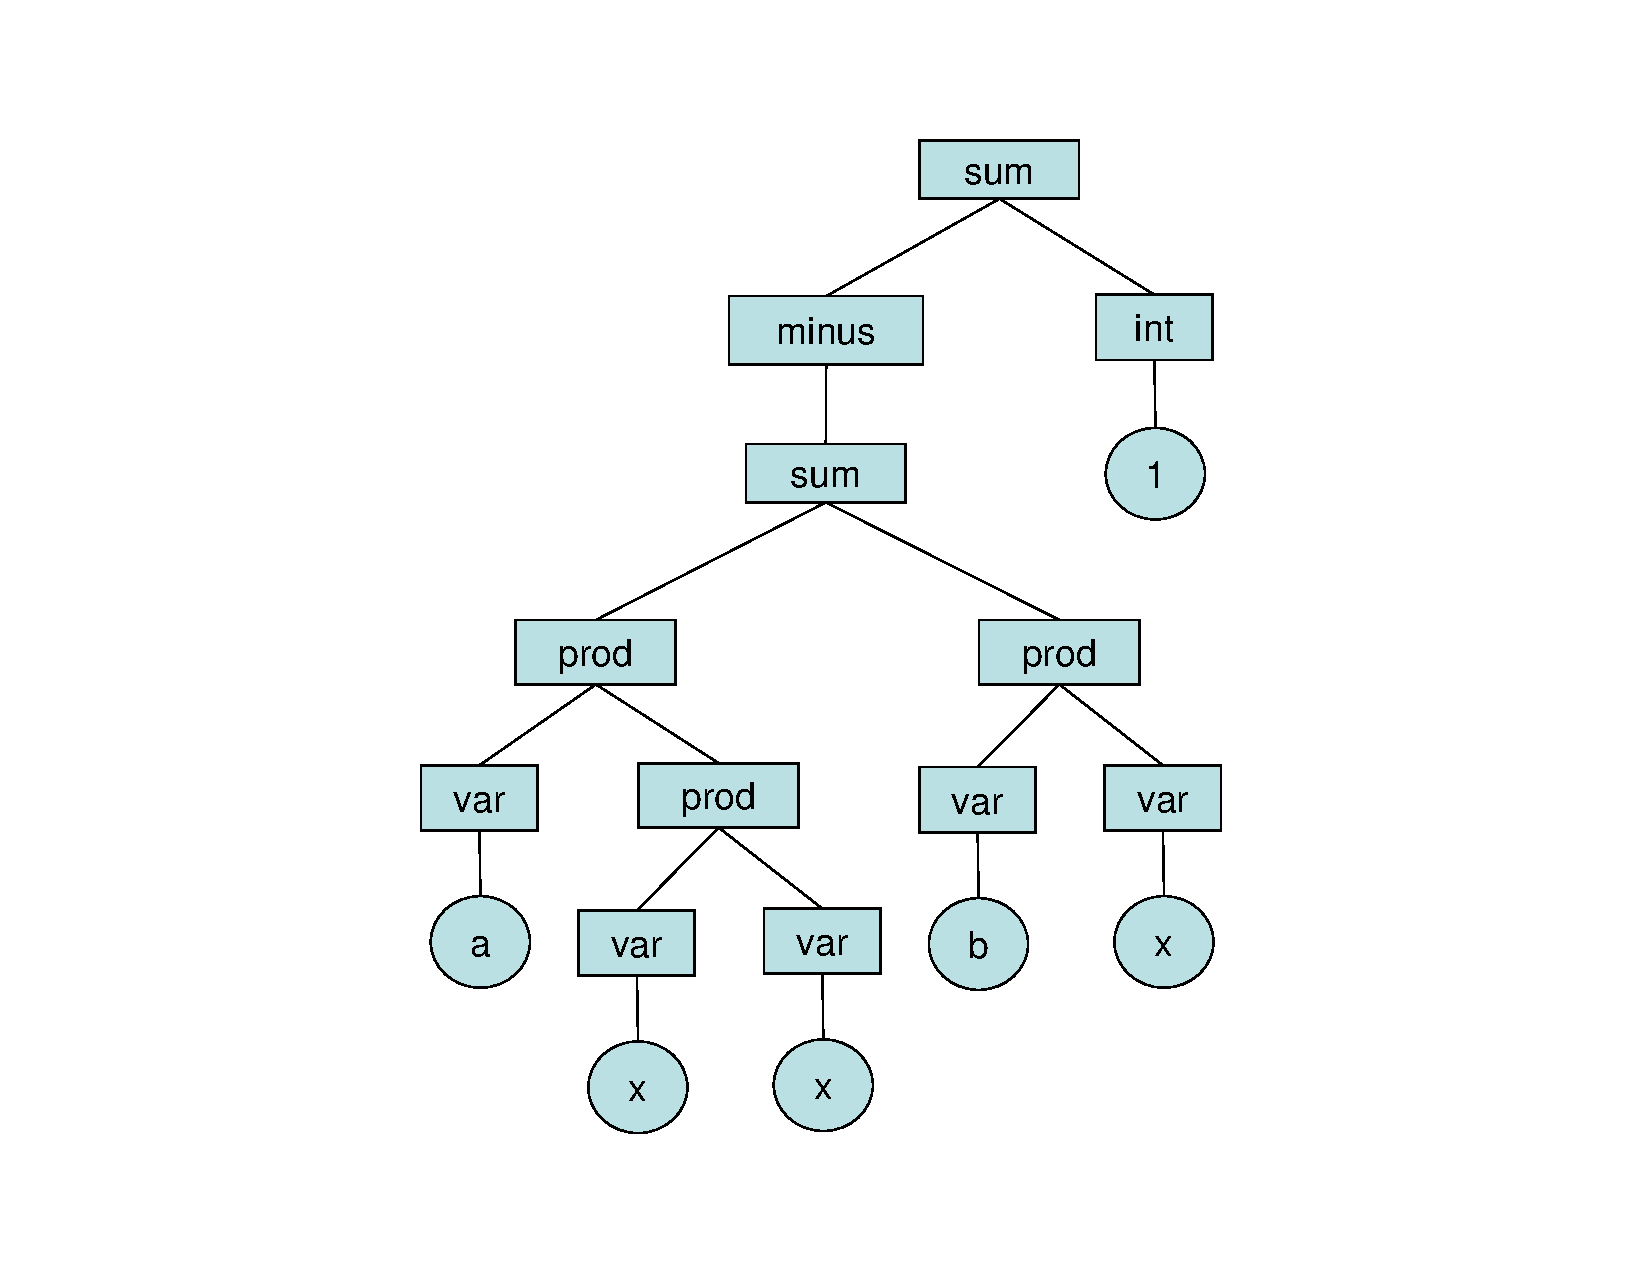
\includegraphics[height=4.5in]{figures/parsetree.pdf}
\caption{Parse tree for $-(a(x\cdot x)+ bx) + 1$.}
\label{fig:parse}
\end{figure}


Such a tree would be represented by pairs or triples that begin with a
\emph{tag} equal to the label of the top node of the parse tree.  We'll
call these tagged data items $\aexp$'s.  
\fi


\subsection{Evaluation and Substitution with Aexp's}

\subsubsection{Evaluating Aexp's}

Since the only variable in an \aexp\ is $x$, the value of an \aexp\ is
determined by the value of $x$.  For example, if the value of $x$ is 3,
then the value of $3x^2 + 2x + 1$ is obviously 34.  In general, given any
$\aexp$, $e$, and an integer value, $n$, for the variable, $x$, we can
evaluate $e$ to finds its value, $\meval(e,n)$.  It's easy, and useful, to
specify this evaluation process with a recursive definition.

\begin{definition}\label{meval-def}
  The \term{evaluation function}, $\meval: \aexp \times \integers \to
  \integers$, is defined recursively on expressions, $e \in \aexp$, as
  follows.  Let $n$ be any integer.

\begin{itemize}
\item \textbf{Base cases:}

\begin{enumerate}

\item\label{eval-var} Case[$e$ is $x$]
\[
\meval(x, n) \eqdef n.
\]
(The value of the variable, $x$, is given to be $n$.)

\item\label{eval-const} Case[$e$ is $\mtt{k}$]
\[
\meval(\mtt{k}, n) \eqdef k.
\]
(The value of the numeral $\mtt{k}$ is the integer $k$, no matter what
value $x$ has.)

\end{enumerate}

\item \textbf{Constructor cases:}

\begin{enumerate}
\setcounter{enumi}{2}

\item\label{eval-sum} Case[$e$ is $(e_1 \sumsym e_2)$]
\[
\meval((e_1 \sumsym e_2),n) \eqdef
  \meval(e_1,n)+\meval(e_2,n).
\]

\item\label{eval-prod} Case[$e$ is $(e_1 \prodsym e_2)$]
\[
\meval((e_1 \prodsym e_2),n) \eqdef \meval(e_1,n) \cdot \meval(e_2,n).
\]

\item\label{eval-minus} Case[$e$ is $\minussym(e_1)$]
\[
\meval(\minussym(e_1),n) \eqdef - \meval(e_1,n).
\]
\end{enumerate}

\end{itemize}

\end{definition}

For example, here's how the recursive definition of $\meval$ would arrive at
the value of $3+x^2$ when $x$ is 2:
\begin{align*}
\meval((\mtt{3} \sumsym (x \prodsym x)),2)
 & = \meval(\mtt{3},2) + \meval((x \prodsym x),2)
                  & \text{(by~Def~\ref{meval-def}.\ref{eval-sum})}\\
 & = 3 + \meval((x \prodsym x),2) & \text{(by~Def~\ref{meval-def}.\ref{eval-const})}\\
 & = 3 + (\meval(x,2) \cdot \meval(x,2)) & \text{(by~Def~\ref{meval-def}.\ref{eval-prod})}\\
 & = 3 + (2 \cdot 2) & \text{(by~Def~\ref{meval-def}.\ref{eval-var})}\\
 & = 3 + 4 = 7.
\end{align*}

\subsubsection{Substituting into Aexp's}
Substituting expressions for variables is a standard, important
operation.  For example the result of substituting the expression $3x$ for $x$
in the $(x(x-1))$ would be $(3x(3x-1)$.  We'll use the general
notation $\msubst{f}{e}$ for the the result of substituting an $\aexp$, $f$,
for each of the $x$'s in an $\aexp$, $e$.  For instance,
\[
\msubst{3x}{x(x-1)} = 3x(3x-1).
\]

This substitution function has a simple recursive definition:

\begin{definition}\label{subst-def}
  The \term{substitution function} from $\aexp \times \aexp$ to \aexp\ is
  defined recursively on expressions, $e \in \aexp$, as follows.  Let $f$
  be any $\aexp$.

\begin{itemize}
\item \textbf{Base cases:}

\begin{enumerate}

\item\label{subst-var} Case[$e$ is $x$]
\[
\msubst{f}{x} \eqdef f.
\]
(The result of substituting $f$ for the variable, $x$, is just $f$.)

\item\label{subst-const} Case[$e$ is $\mtt{k}$]
\[
\msubst{f}{\mtt{k}} \eqdef \mtt{k}.
\]
(The numeral, $\mtt{k}$, has no $x$'s in it to substitute for.)

\end{enumerate}

\item \textbf{Constructor cases:}

\begin{enumerate}
\setcounter{enumi}{2}
\item\label{subst-sum} Case[$e$ is $(e_1 \sumsym e_2)$]
\[
\msubst{f}{(e_1 \sumsym e_2)}) \eqdef  (\msubst{f}{e_1} \sumsym
\msubst{f}{e_2}).
\]

\item\label{subst-prod} Case[$e$ is $(e_1 \prodsym e_2)$]
\[
\msubst{f}{(e_1 \prodsym e_2)}) \eqdef  (\msubst{f}{e_1} \prodsym
\msubst{f}{e_2}).
\]

\item\label{subst-minus} Case[$e$ is $\minussym(e_1)$]
\[
\msubst{f}{\minussym(e_1)} \eqdef \minussym (\msubst{f}{e_1}).
\]

\end{enumerate}
\end{itemize}
\end{definition}

Here's how the recursive definition of the substitution function would find
the result of substituting $3x$ for $x$ in the $x(x-1)$:
\begin{align*}
\msubst{3x}{(x(x-1))} & =
\msubst{3x}{(x \prodsym (x \sumsym \minussym(1)))} & \text{(unabbreviating)}\\
 & = (\msubst{3x}{x} \prodsym \msubst{3x}{(x \sumsym \minussym(1))})
         & \text{(by~Def~\ref{subst-def}~\ref{subst-prod})}\\
 & = (3x \prodsym \msubst{3x}{(x \sumsym \minussym(1))})
         & \text{(by~Def~\ref{subst-def}~\ref{subst-var})}\\
 & = (3x \prodsym (\msubst{3x}{x} \sumsym \msubst{3x}{\minussym(1)}))
         & \text{(by~Def~\ref{subst-def}~\ref{subst-sum})}\\
 & = (3x \prodsym (3x \sumsym \minussym (\msubst{3x}{1})))
         & \text{(by~Def~\ref{subst-def}~\ref{subst-var} \&~\ref{subst-minus})}\\
 & = (3x \prodsym (3x \sumsym \minussym (1)))
         & \text{(by~Def~\ref{subst-def}~\ref{subst-const})}\\
 & = 3x(3x-1) & \text{(abbreviation)}
\end{align*}

Now suppose we have to find the value of $\msubst{3x}{(x(x-1))}$ when $x =
2$.  There are two approaches.

First, we could actually do the substitution above to get $3x(3x-1)$, and
then we could evaluate $3x(3x-1)$ when $x =2$, that is, we could
recursively calculate $\meval(3x(3x-1),2)$ to get the final value 30.  In
programming jargon, this would be called evaluation using the
\emph{Substitution Model}.  Tracing through the steps in the evaluation,
we find that the Substitution Model requires two substitutions for
occurrences of $x$ and 5 integer operations: 3 integer multiplications, 1
integer addition, and 1 integer negative operation.  Note that in this
Substitution Model the multiplication $3 \cdot 2$ was performed twice to
get the value of 6 for each of the two occurrences of $3x$.

The other approach is called evaluation using the \emph{Environment
  Model}.  Namely, we evaluate $3x$ when $x = 2$ using just 1
multiplication to get the value 6.  Then we evaluate $x(x-1)$ when $x$ has
this value 6 to arrive at the value $6\cdot 5=30$.  So the Environment
Model requires 2 variable lookups and only 4 integer operations: 1
multiplication to find the value of $3x$, another multiplication to find
the value $6 \cdot 5$, along with 1 integer addition and 1 integer
negative operation.

So the Environment Model approach of calculating
\[
\meval(x(x-1), \meval(3x,2))
\]
instead of the Substitution Model approach of calculating
\[
\meval(\msubst{3x}{x(x-1)},2)
\]
is faster.  But how do we know that these final values reached by these
two approaches always agree?  We can prove this easily by structural
induction on the definitions of the two approaches.  More precisely, what
we want to prove is

\begin{theorem}\label{environments}
For all expressions $e,f \in \aexp$ and $n \in \integers$,
\begin{equation}\label{eval-subst}
\meval(\msubst{f}{e},n) = \meval(e, \meval(f,n)).
\end{equation}
\end{theorem}

\begin{proof}
The proof is by structural induction on $e$.\footnote{This is an example
of why it's useful to notify the reader what the induction variable is
---in this case it isn't $n$.}

\textbf{Base cases:}
\begin{itemize}

\item Case[$e$ is $x$]

  The left hand side of equation~\eqref{eval-subst} equals $\meval(f,n)$
  by this base case in Definition~\ref{subst-def} of the substitution
  function, and the right hand side also equals $\meval(f,n)$ by this base
  case in Definition~\ref{meval-def} of $\meval$.


\item Case[$e$ is $\mtt{k}$].

  The left hand side of equation~\eqref{eval-subst} equals $\mtt{k}$ by
  this base case in Definitions~\ref{subst-def} and~\ref{meval-def} of
  the substitution and evaluation functions.  Likewise, the right hand
  side equals $\mtt{k}$ by two applications of this base case in the
  Definition~\ref{meval-def} of $\meval$.

\end{itemize}

\textbf{Constructor cases}:
\begin{itemize}

\item Case[$e$ is $(e_1 \sumsym e_2)$]

  By the structural induction hypothesis~\eqref{eval-subst}, we may assume
  that for all $f \in \aexp$ and $n \in \integers$,

\begin{equation}\label{ln4.hyp}
\meval(\msubst{f}{e_i},n)  =  \meval(e_i, \meval(f,n))
\end{equation}
for $i= 1,2$.  We wish to prove that

\begin{equation}\label{s+}
\meval(\msubst{f}{(e_1\sumsym e_2)},n)  =  \meval((e_1 \sumsym e_2), \meval(f,n))
\end{equation}

But the left hand side of~(\ref{s+}) equals
\[
\meval(\, (\msubst{f}{e_1} \sumsym \msubst{f}{e_2}),\ n)
\]
by Definition~\ref{subst-def}.\ref{subst-sum} of substitution into a sum
expression.  But this equals
\[
\meval(\msubst{f}{e_1},n) + \meval(\msubst{f}{e_2},n)
\]
by Definition~\ref{meval-def}.\ref{eval-sum} of $\meval$ for a sum expression.  By
induction hypothesis~\eqref{ln4.hyp}, this in turn equals
\[
\meval(e_1,\meval(f,n)) + \meval(e_2,\meval(f,n)).
\]
Finally, this last expression equals the right hand side of~(\ref{s+}) by
Definition~\ref{meval-def}.\ref{eval-sum} of $\meval$ for a sum
expression.  This proves~(\ref{s+}) in this case.

\item $e$ is $(e_1 \prodsym e_2)$.  Similar.

\item $e$ is $-(e_1)$.  Even easier.

\end{itemize}

This covers all the constructor cases, and so completes the proof by
structural induction.

\end{proof}


\iffalse
\subsection{A String Theorem}

Here is a more complex proof, illustrating a combination of structural
induction and strengthening the hypothesis.

\begin{theorem}
  In a string of $0$s and $1$s, the number of occurrences of the pattern
  $01$ is less than or equal to the number of occurrences of $10$, plus
  one.
\end{theorem}

Let's try to prove this by structural induction.  First we must
define $P(s)$.  Let's write $\ms{num}(pat,s)$ as the number of
occurrences of the pattern string pat in s.  Now our inductive
hypothesis is
\[
P(s): \ms{num}(01,s) \leq \ms{num}(10,s) + 1. 
\]
If you try to prove this by structural induction, you will get
stuck.
Why? 
Consider what happens when you add $1$ at the end.  
This could increase the number of $01$s without increasing the number of
$10$s. 

So, to prove by structural induction on strings, let's strengthen the
hypothesis by adding another clause.  If a string ends in $0$ then
the number of $01$s is less than or equal to the number of $10$s.
That solves the problem by weakening what we have to show when the
string ends in $1$.  But maybe it causes another problem somewhere
else.  Let's give it a try:

Redefine $P(s) \eqdef$
\begin{eqnarray*}
\ms{num}(01,s) & \leq & \ms{num}(10,s) + 1, \text{ and}\\
\leftenq{\text{If $s$ ends in $0$ then}}\\
\ms{num}(01,s) & \leq  &\ms{num}(10,s).
\end{eqnarray*} 
 
This means that, for each inductive step have two things to show.

\structuredproof{

  Prove: $\forall s \in S \; (P(s))$ \\
  1. (Base) $P(\emptystring)$ 
  \reason{No patterns of either kind.} \\
  2. (Inductive step) $\forall s \in S \; (P(s) \implies P(s 0))$ \\
  1. Fix $s$. \\
  2. Assume $P(s)$. \\
  3. $P(s 0)$ \\
  1. $\ms{num}(01,s0) \leq \ms{num}(10,s0) + 1$. 
  \reason{???} \\
  2. If $s 0$ ends in $0$ then $\ms{num}(01,s0) \leq
  \ms{num}(10,s0)$. \noreason \\
  \reason{???} \\
  3. QED
  \reason{Conjunction} \\
  4. QED 
  \reason{Implication, UG} \\
  3. (Inductive step) $\forall s \in S \; (P(s) \implies P(s 1))$ \\
  1. Fix $s$. \\
  2. Assume $P(s)$. \\
  3. $P(s 1)$ \\
  1. $\ms{num}(01,s1) \leq \ms{num}(10,s1) + 1$. 
  \reason{???} \\
  2. If $s 1$ ends in $0$ then $\ms{num}(01,s1) \leq
  \ms{num}(10,s1)$.\noreason \\
  \reason{???} \\
  3. QED
  \reason{Conjunction} \\
  4. QED 
  \reason{Implication, UG} \\
  4. QED
  \reason{Structural induction on strings.}\\
}

First let's consider $s1$. This is the case that looks dangerous,
because it might increase the number of $01$s.  We have to prove two
statements.  The second is easy, because the new string doesn't end in
$0$.  We say it's ``vacuously true''.

The first statement now takes some work. 
We might be adding to the number of $01$s.  
However, if we do, the previous string must have ended with $0$. 
Then the inductive hypothesis says that the previous string had to
satisfy the stronger inequality in the second statement. 
Adding one to the LHS of the stronger inequality yields the weaker
inequality we want.

The following proof fragment considers cases based on whether $s$ ends
in $0$ or not.  If not, it might end in $1$, or might be empty (don't
forget this possibility).

\begin{proof}
  3. $P(s 1)$ \\
  1. $\ms{num}(01,s1) \leq \ms{num}(10,s1) + 1$. \\
  1. If $s$ ends in $0$ then $\ms{num}(01,s1) \leq\ms{num}(10,s1) + 1$. \\
  1. Assume $s$ ends in $0$. \\
  2. $\ms{num}(01,s) \leq \ms{num}(10,s)$ 
  Inductive hypothesis (3.2), part 2. \\
  3. $\ms{num}(01,s1) = \ms{num}(01,s) + 1$ 
  Adding one more $01$. \\
  4. $\ms{num}(10,s1) = \ms{num}(10,s)$ \\
  5. $\ms{num}(01,s1) \leq\ms{num}(10,s1) + 1$. 
  Algebra (combining 3.3.1.1.2, ...3, and ...4) \\
  QED 
  Implication \\
  2. If $s$ ends in $1$ then $\ms{num}(01,s1)\leq\ms{num}(10,s1) + 1$. \\
  Inductive hypothesis, part 1; no new $01$s. \\
  3. If $s = \emptystring$ then $\ms{num}(01,s1) \leq\ms{num}(10,s1)+ 1$. \\
  $s1$ is just $1$, which has no $01$s. \\
  4. QED 
  Cases \\
  2. If $s 1$ ends in $0$ then $\ms{num}(01,s1) \leq \ms{num}(10,s1)$. \\
  Vacuously true, because $s1$ doesn't end in $0$. \\
  3. QED
  Conjunction \\
\end{proof}
Of course, you could also expand the step for $s$ ending in $1$ into a
careful series of inequalities.

Now consider $s0$.  We hope that what we did to make the $s1$ case
work doesn't mess up the $s0$ case.  But we have to check.

The first statement is easy.  It follows from the first statement of
the inductive hypothesis for $s$, because we are not increasing the
number of $01$s.  But now the second statement takes more work.  The
difficulty is that the new string ends in $0$, which means that we
have to show the stronger inequality in the second statement.  But to
do this, we might only have the weaker inequality for the previous
string.  The argument again depends on what the previous string $s$
ended with.  So again, we consider cases, based on whether $s$ ends in
$0$ or $1$, or is empty.  If $s$ ends in $0$ we rely on the second
statement of the inductive hypothesis for $s$ (with the stronger
inequality), whereas if $s$ ends in $1$ we rely on the first statement
(with the weaker inequality).  In this case, we have to ``turn the
weaker inequality into the stronger inequality''.

\structuredproof[38ex]{
  3. $P(s 0)$ \\
  1. $\ms{num}(01,s0) \leq \ms{num}(10,s0) + 1$.
  \reason{Induct. hypothesis, part 1; no new $01$s.} \\
  2. If $s 0$ ends in $0$ then $\ms{num}(01,s0) \leq\ms{num}(10,s0)$. \\
  1. $\ms{num}(01,s0) \leq \ms{num}(10,s0)$. \\
  1. If $s$ ends in $0$ then $\ms{num}(01,s0)
  \leq\ms{num}(10,s0)$. \noreason \\
  \reason{Induct. hypothesis, part 2; no new $01$s} \\
  2. If $s$ ends in $1$ then $\ms{num}(01,s0)
  \leq\ms{num}(10,s0)$. \noreason \\ 
  1. Assume $s$ ends in $1$. \\
  2. $\ms{num}(01,s) \leq \ms{num}(10,s) + 1$. 
  \reason{Inductive hypothesis, part 1} \\
  3. $\ms{num}(01,s0) = \ms{num}(01,s)$ \\
  4. $\ms{num}(10,s0) = \ms{num}(10,s) + 1$ 
  \reason{Exactly one new occurrence of $10$.} \\
  5. $\ms{num}(01,s0) \leq \ms{num}(10,s0)$ 
  \reason{Algebra} \\
  6. QED
  \reason{Implication} \\
  3. If $s = \emptystring$ then $\ms{num}(01,s0) \leq
  \ms{num}(10,s0)$. \noreason \\ 
  
\reason{$s0$ is just $1$, which has no $01$s or $10$s.} \\
  4. QED 
  \reason{Cases} \\
  2. QED
  \reason{Propositional reasoning (truth table)} \\
  3. QED 
  \reason{Conjunction}\\
}

If you actually write out all these cases in the proof, you will
notice that some facts are stated repeatedly, e.g., that when you add
a $0$ to the end of a string you are not increasing the number of
$01$s.  To avoid having to state these facts several times, you can
move them earlier in the proof.
\fi


\iffalse

\begin{example*}
\begin{definition}\label{E}
Define a set, $E$, recursively as follows:
\begin{itemize}
\item \textbf{Base case:} $0 \in E$,\label{0E}
\item \textbf{Constructor cases:} if $n \in E$, then
\begin{enumerate}
\item $n+2 \in E$, when $n\geq 0$;\label{+2E}
\item $-n \in E$, when $n > 0$.\label{-E}
\end{enumerate}
\end{itemize}

\end{definition}
\end{example*}

Using this definition, we can see that $0 \in E$ by the Base case, so $0 +
2 = 2 \in E$ by Constructor case~\ref{+2E}., and so $2+2 =4 \in E$, $4+2 =
6 \in E$, \dots, and in fact any nonnegative even number is in $E$ by
successive application of case~\ref{+2E}.  Also, by case~\ref{-E}.,
$-2,-4,-6,\dots \in E$.  So clearly all the even integers are in $E$.

Is anything else in $E$?  The definition doesn't say so explicitly, but an
implicit condition on a recursive definition is that the only way things
get into $E$ is as a consequence of the Base and Constructor cases.  In
other words, $E$ will be exactly the set of even integers.

A very simple application of structural induction proves that the set $E$
given by Definition~\ref{E} is exactly the set of even numbers.  We already
explained why all the even numbers are in $E$.  So what's left is to show
that:

\begin{lemma*}
Every number in the set $E$ in Definition~\ref{E} is even.
\begin{proof}
The proof is by structural induction on $n \in E$.  The induction
hypothesis is 
\[
Q(n) \eqdef \text{$n$ is even}.
\]

\textbf{Base case}: $Q(0)$ holds since 0 is even.

\textbf{Constructor cases}: assuming $n \in E$ and $Q(n)$ holds, prove
that
\begin{itemize}

\item $Q(n+2)$ holds.  This is immediate, since adding 2 to an even number
  gives an even number.

\item $Q(-n)$ holds.  This is also immediate, since $n$ is even iff $-n$ is
even.

\end{itemize}

This completes the proof of the Constructor cases, and we conclude by
structural induction at $Q(n)$ holds for all $n \in E$.
\end{proof}

\end{lemma*}


defining the set, $E$, of even numbers as in Definitions~\ref{E}, but
without the conditions~\ref{+2E}.\ and~\ref{-E}.\ that restrict application of
the rules.  Namely,

\begin{definition}\label{Eamb}
Define a set, $E'$, recursively as follows:
\begin{itemize}
\item \textbf{Base case:} $0 \in E'$,\label{0Eamb}
\item \textbf{Constructor cases:} if $n \in E'$, then
\begin{enumerate}
\item $n+2 \in E'$, \label{+2Eamb}
\item $-n \in E'$.\label{-Eamb}
\end{enumerate}
\end{itemize}
\end{definition}

Now Definition~\ref{Eamb} is perfectly legitimate, and we could us it to
prove by structural induction that $E'$ also is the set of even integers,
that is, $E'= E$.  But Definition~\ref{Eamb} is ambiguous.  For example,
$0\in E'$ by the base case, but also $0=-0 \in E'$ by applying constructor
case~\ref{-Eamb} to the base case.  This begins to matter when we try to
define a function, $s$, from $E'$ to nonnegative integers based on
Definition~\ref{Eamb}:
\begin{align*}
  s(0) & \eqdef 1,\\
s(n+2) & \eqdef 1+ s(n),\\
 s(-n) & \eqdef 1+ s(n).
\end{align*}
So $s(0) \eqdef 1$ by the base case of this definition, and also $s(0)=
s(-0) \eqdef 1+s(0) = 1 + 1 = 2$ by the second constructor case, which
shows that these rules are inconsistent.

On the other hand, using the unambiguous Definition~\ref{E} of $E$,
essentially the same definition of $S$ works just fine.  Namely, define
\begin{align*}
  s(0) & \eqdef 1,\\
  s(n+2) & \eqdef 1+ s(n), & \text{ for } n \geq 0\\
  s(-n) & \eqdef 1+ s(n) & \text{ for } n > 0.
\end{align*}
Now $s(n)$ is unambiguously defined, and in fact is precisely the (unique)
number of steps required to construct $n \in E$ according to the
unambiguous Definition~\ref{E} of $E$.
\fi

%% Structural Induction on Recursive Data Types Problems %%%%%%%%%%%%%%%%%%%%%%
%\startclassproblems
\pinput{CP_F18_functions}
\pinput{CP_recursively_defined_sets}
\pinput{CP_erasable_strings}
\pinput{CP_binary_trees}


%% Games as a Recursive Data Type %%%%%%%%%%%%%%%%%%%%%%%%%%%%%%%%%%%%%%%%%%%%%
\section{Games as a Recursive Data Type}

Chess, Checkers, and Tic-Tac-Toe are examples of \emph{two-person
terminating games of perfect information}, ---$\tg$'s for short.  These
are games in which two players alternate moves that depend only on the
visible board position or state of the game.  ``Perfect information''
means that the players know the complete state of the game at each move.
(Most card games are \emph{not} games of perfect information because
neither player can see the other's hand.)  ``Terminating'' means that play
cannot go on forever ---it must end after a finite number of
moves.\footnote{Since board positions can repeat in chess and checkers,
termination is enforced by rules that prevent any position from being
repeated more than a fixed number of times.  So the ``state'' of these
games is the board position \emph{plus} a record of how many times
positions have been reached.}

We will define $\tg$'s \iffalse in a straightforward way tagged\fi as a 
recursive data type.  To see how this will work, let's use the game of
Tic-Tac-Toe as an example.

\subsection{Tic-Tac-Toe}

Tic-Tac-Toe is a game for young children.  There are two players who
alternately write the letters ``X'' and ``O'' in the empty boxes of a $3
\times 3$ grid.  Three copies of the same letter filling a row, column, or
diagonal of the grid is called a \emph{tic-tac-toe}, and the first player
who gets a tic-tac-toe of their letter wins the game.  \iffalse Children
generally don't take long to figure out an optimal strategy for playing the
game.\fi


We're now going give a precise mathematical definition of the Tic-Tac-Toe
\term{game tree} as a recursive data type.  \iffalse and carefully defining
the allowed moves Children of course have no need for such a definition,
and it would be too complicated for them anyway.  But if we had to write a
Tic-Tac-Toe playing \emph{computer program}, we'd need this kind of picky
precision.\fi Here's the idea behind the definition: at any point in the
game, the ``board position'' is the pattern of X's and O's on the $3 \times
3$ grid.  From any such Tic-Tac-Toe pattern, there are a number of next
patterns that might result from a move.  For example, from the initial
empty grid, there are nine possible next patterns, each with a single X in
some grid cell and the other eight cells empty.  From any of these
patterns, there are eight possible next patterns gotten by placing an O in
an empty cell.  These move possibilities are given by the
\hyperdef{game}{tree}{game tree} for Tic-Tac-Toe indicated in
Figure~\ref{fig:Tic-Tac-Toe}.

\begin{figure}[htbp]
\centering
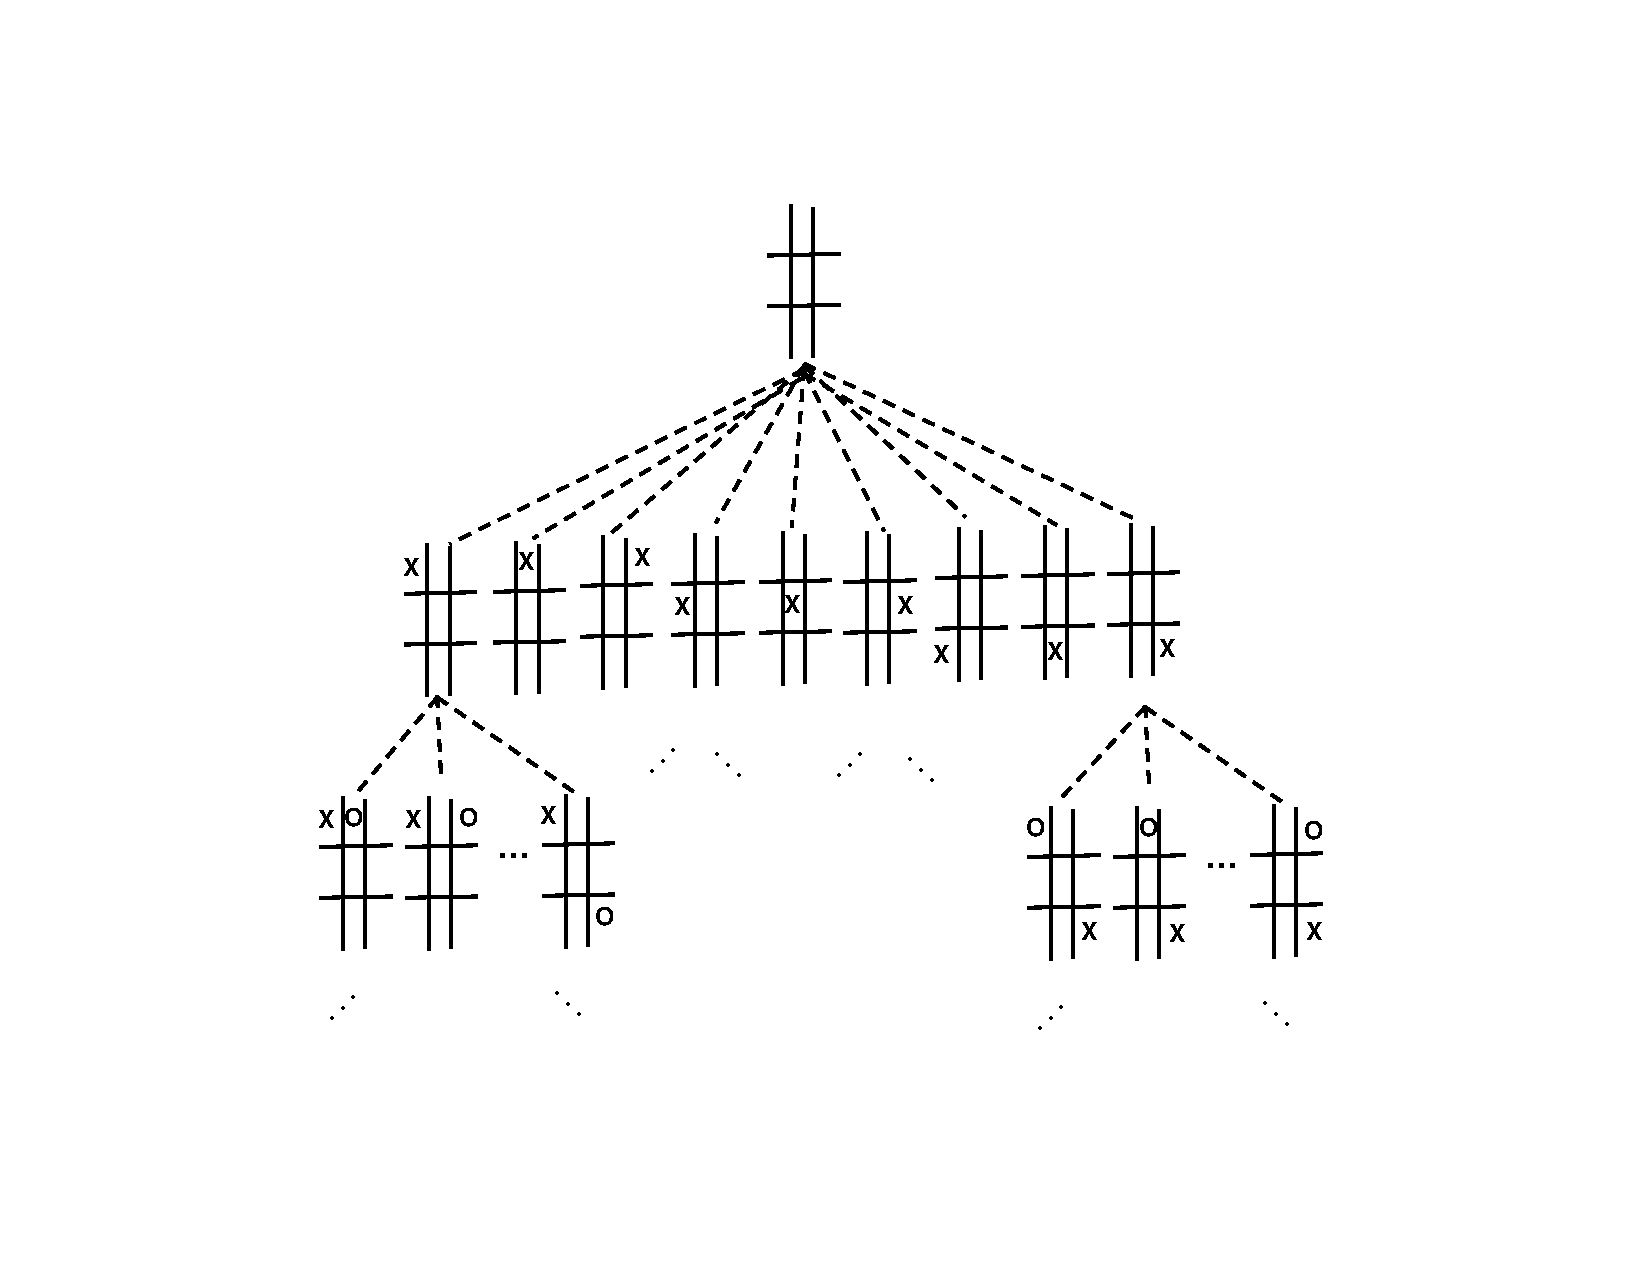
\includegraphics[height=6in]{figures/topgame.pdf}
\caption{The Top of the Game Tree for Tic-Tac-Toe.}
\label{fig:Tic-Tac-Toe}
\end{figure}


\iffalse
\[\begin{array}{c|c|c}
\hspace{.1in} & \hspace{.1in} & \hspace{.1in}\\
\hline  & &\\
\hline  & &
\end{array}\]

\textbf{FIGURE NEEDED}
\fi

\begin{definition}

A Tic-Tac-Toe \emph{pattern} is a $3 \times 3$ grid each of whose 9 cells
contains either the single letter, X, the single letter, O, or is
empty.
\iffalse
Moreover, there must be either
\begin{itemize}

\item one more X than O's, with at most two tic-tac-toes of X's, and no
tic-tac-toe of O's, or

\item an equal number of X's and O's, with at most one tic-tac-toes of
O's, and no tic-tac-toe of X's.
\end{itemize}
\fi

A pattern, $Q$, is a \emph{possible next pattern after} $P$, providing $P$
has no tic-tac-toes and
\begin{itemize}

\item if $P$ has an equal number of X's and O's, and $Q$ is the same as
$P$ except that a cell that was empty in $P$ has an X in $Q$, or

\item if $P$ has one more X than O's, and $Q$ is the same as $P$ except
that a cell that was empty in $P$ has an O in $Q$.
\end{itemize}

If $P$ is a Tic-Tac-Toe pattern, and $P$ has no next patterns, then the
\emph{terminated Tic-Tac-Toe game trees} at $P$ are

\begin{itemize}

\item 
\[
\ang{P, \ang{\texttt{win}}},
\]
if $P$ has a tic-tac-toe of X's.


\item 
\[
\ang{P, \ang{\texttt{lose}}},
\]
if $P$ has a tic-tac-toe of O's.


\item
\[
\ang{P, \ang{\texttt{tie}}},
\]
otherwise.

\end{itemize}


\iffalse
If $Q$ is a possible move from $P$, then the game tree starting at $Q$ is
called a \emph{  Notice
that $\mathcal{G}_P = \emptyset$ iff $P$ is terminated.}
\fi

The \emph{Tic-Tac-Toe game trees starting at $P$} are defined recursively:

\textbf{Base Case}:
A terminated Tic-Tac-Toe game tree at $P$ is a Tic-Tac-Toe game tree
starting at $P$.

\textbf{Constructor case}: If $P$ is a non-terminated Tic-Tac-Toe pattern,
then the Tic-Tac-Toe game tree starting at $P$ consists of $P$ and the set
of all games trees starting at possible next patterns after $P$.
\end{definition}

For example, if
\begin{align*}
P_0 & =  \begin{array}{c|c|c}
                O & X & O\\
         \hline X & O & X\\
         \hline X & &
        \end{array}\\
Q_1 & = \begin{array}{c|c|c}
                O & X & O\\
         \hline X & O & X\\
         \hline X &  & O
        \end{array}\\
Q_2 & = \begin{array}{c|c|c}
                O & X & O\\
         \hline X & O & X\\
         \hline X & O & 
        \end{array}\\
R & = \begin{array}{c|c|c}
                O & X & O\\
         \hline X & O & X\\
         \hline X & O & X
        \end{array}
\end{align*}
the game tree starting at $P_0$ is pictured in Figure~\ref{fig:endgame}.

\iffalse
Then,
\begin{equation}\label{endgame}
\ang{P, \set{\ang{Q_1, \ang{\texttt{lose}}},
             \ang{Q_2, \set{\ang{R,\ang{\texttt{tie}}}}}}}
\end{equation}
is the tagged recursive datum that corresponds to a Tic-Tac-Toe ``end
game'' that starts with $P$.  This game is easier to understand by looking
at its game tree in Figure~\ref{fig:endgame}.  Notice that the game tree
---which so far we haven't actually defined ---is simply the parse tree of
the tagged datum.\fi


\begin{figure}[htbp]
\centering
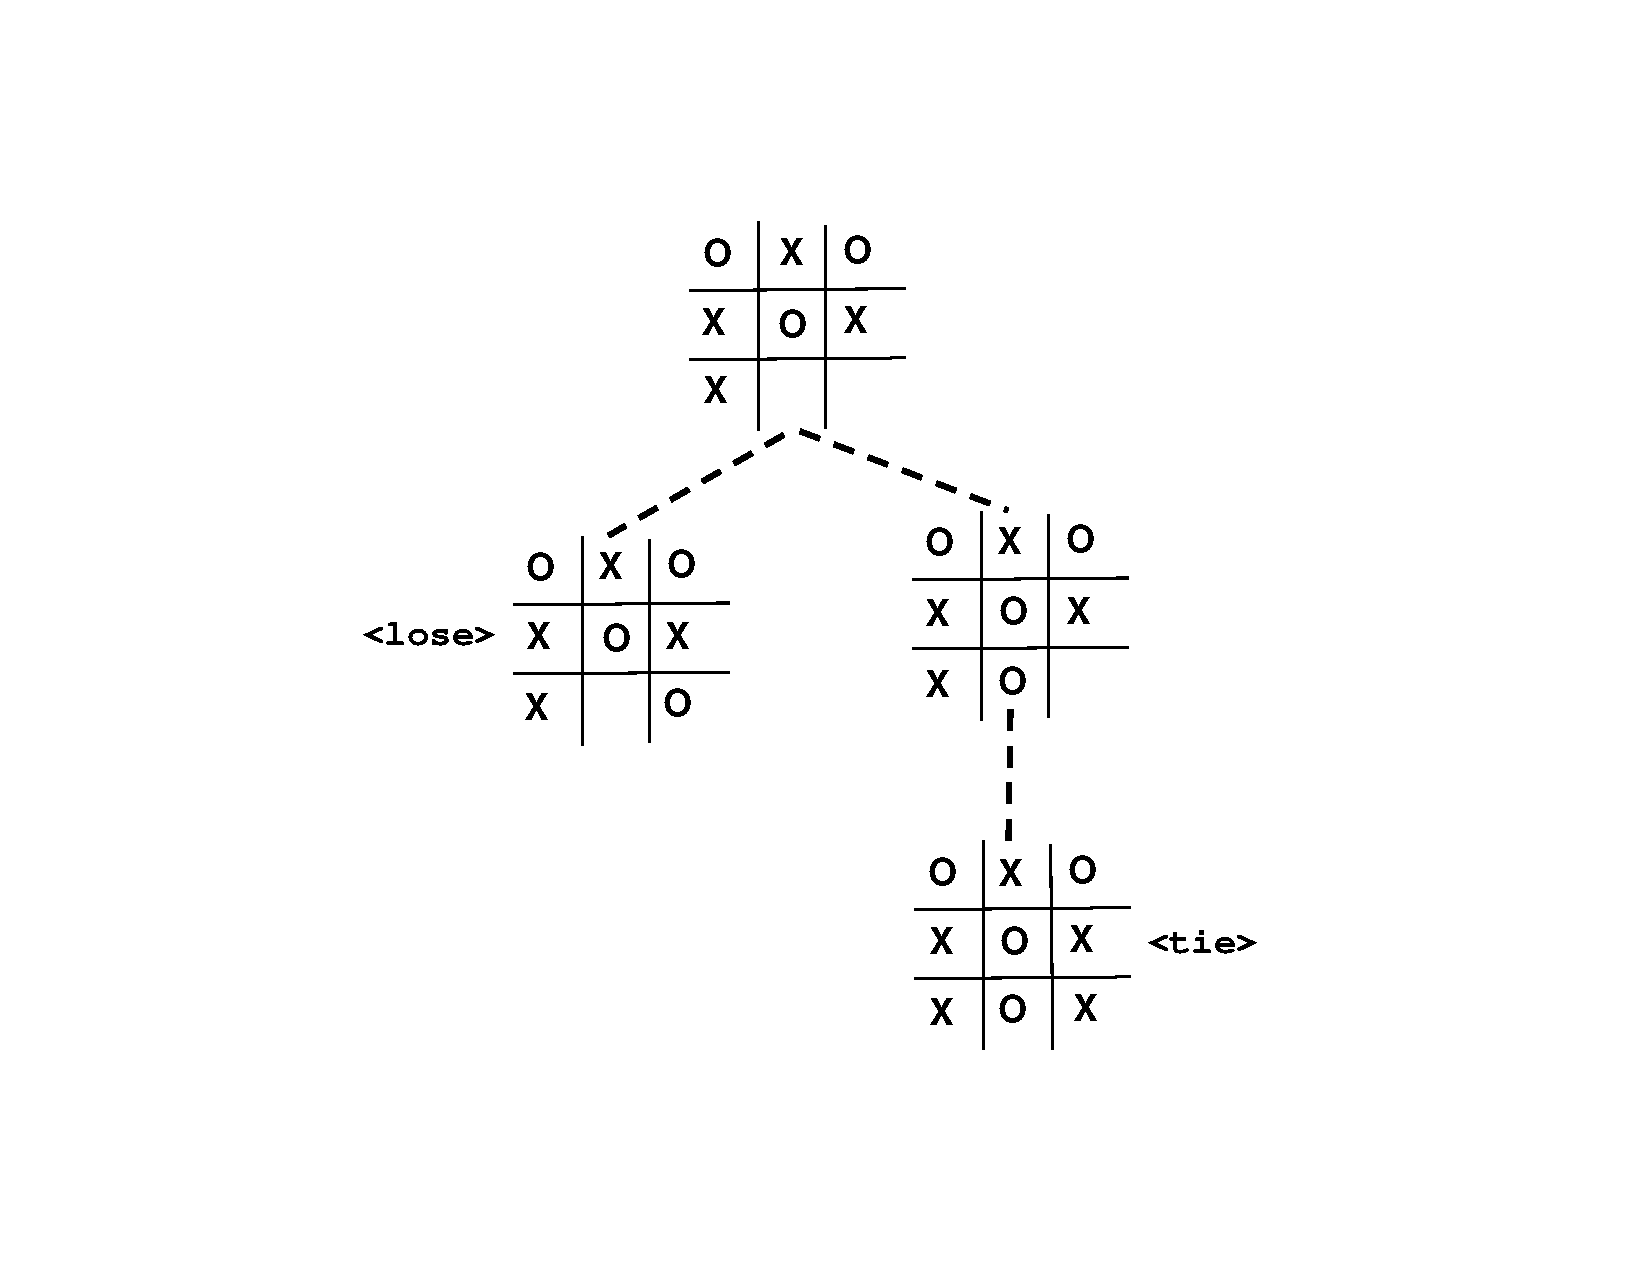
\includegraphics[height=4in]{figures/endgame.pdf}
\caption{Game Tree for the Tic-Tac-Toe game starting at $P_0$.}
\label{fig:endgame}
\end{figure}

Game trees are usually pictured in this way with the starting pattern
(referred to as the ``root'' of the tree) at the top and lines connecting
the root to the \iffalse roots of the \fi game trees that start at each
possible next pattern.  The ``leaves'' at the bottom of the tree (trees
grow upside down in Computer Science) correspond to terminated games.  A
path from the root to a leaf describes a complete \emph{play} of the game.
(In English, ``game'' can be used in two senses: first we can say that
Chess is a game, and second we can play a game of Chess.  The first usage
refers to the data type of Chess game trees, and the second usage refers to
a ``play.'')

\subsection{Infinite Tic-Tac-Toe Games}

At any point in a Tic-Tac-Toe game, there are at most nine possible next
patterns, and no play can continue for more than nine moves.  But suppose
we consider an \emph{$n$-game Tic-Tac-Toe tournament} where the tournament
winner is the one who wins more of $n>0$ individual Tic-Tac-Toe games.  (If
they each win an equal number of individual games, then the tournament is a
tie.)

Now we can consolidate all these tournaments into a single game we can call
\emph{Tournament-Tic-Tac-Toe}: the first player in Tournament-Tic-Tac-Toe
chooses any integer $n > 0$, and then the players play an $n$-game
tournament.  Now there are infinitely many possible first moves: the first
player can choose $n=1$, or $n=2$, or $n=3$, or \dots.  But still, it's
obvious that every possible play of Tournament-Tic-Tac-Toe is finite,
because after the first player chooses a value for $n$, the game can't
continue for more than $9n$ moves.  So it's not possible to keep playing
forever even though the game tree is infinite.

This isn't very hard to understand, but there is an important difference
between any given $n$-game tournament and Tournament-Tic-Tac-Toe: even
though every play of Tournament-Tic-Tac-Toe must come to an end, there is
no longer any bound on how many moves it might be before the game ends ---a
play might end after 9 moves, or $9(2001)$ moves, or $9(10^{10}+1)$ moves;
it just can't continue forever.

\iffalse While there is no bound on how long to play, at least after the
first move to an $n \times n$ board in meta-Tic-Tac-Toe, we know the game
will end with $n^2$ moves.\fi

With Tournament-Tic-Tac-Toe recognized as a \tg, we can go on to
Tournament$^2$-Tic-Tac-Toe where the first player chooses a number, $m>0$,
of Tournament-Tic-Tac-Toe games to play, and the second player acts as the
first player in each of the $m$ Tournament-Tic-Tac-Toe games to be played.
Then, of course, there's Tournament$^3$-Tic-Tac-Toe\dots.

\iffalse Every play of the meta-meta game must still end, but now even
after the first move, there is no bound on how long a game might
continue.\fi

\subsection{Two Person Terminating Games}

Familiar games like Tic-Tac-Toe, Checkers, and Chess can all end in ties,
but for simplicity we'll only consider win/lose games ---no ``everybody
wins''-type games at MIT. \texttt{:-)}.  But everything we show about
win/lose games will extend easily to games with ties.

\iffalse
Of course Tic-Tac-Toe and the
other games will fit this set up if we treat a game that ends in a tie as
a loss for the usual first player ---White in Chess, Red in Checkers, the
X-player in Tic-Tac-Toe.
\fi

Like Tic-Tac-Toe, the idea behind the definition of $\tg$'s as a recursive
data type is that making a move in a $\tg$ leads to the start of a subgame.
For Tic-Tac-Toe, we used the patterns and the rules of Tic-Tac-Toe to
determine the next patterns.  But once we have a complete game tree, we
don't really need the pattern labels: the root of a game tree itself can
play the role of a ``board position'' with its possible ``next positions''
determined by the roots of its subtrees.  This leads to the following very
simple ---perhaps deceptively simple ---general definition.

\begin{definition}
The \hyperdef{2p}{tg}{$\tg$}, \emph{game trees for two-person terminating
    games of perfect information} are defined recursively as follows:
\begin{itemize}

\item \textbf{Base cases:}
\[\begin{array}{ll}
\ang{\texttt{leaf},\texttt{win}} & \in \tg, \text{ and}\\
\ang{\texttt{leaf},\texttt{lose}}& \in \tg.
\end{array}\]

\item \textbf{Constructor case:}
If $\mathcal{G}$ is a nonempty set of
$\tg$'s, then $G$ is a $\tg$, where
\[
G \eqdef \ang{\texttt{tree},\mathcal{G}}.
\]
The games trees in $\mathcal{G}$ are called the possible \emph{next moves}
from $G$.
\end{itemize}

\end{definition}

These games are called ``terminating'' because, even though a $\tg$ may be
a (very) infinite datum like Tournament$^2$-Tic-Tac-Toe, every play of a
$\tg$ must terminate.  This is something we can now prove, after we give a
precise definition of ``play'':

\begin{definition}
A \emph{play} of a $\tg$, $G$, is a (potentially infinite) sequence of
$\tg$'s starting with $G$ and such that if $G_1$ and $G_2$ are consecutive
$\tg$'s in the play, then $G_2$ is a possible next move of $G_1$.

If a $\tg$ has no infinite play, it is called a \emph{terminating} game.
\end{definition}

\begin{theorem}
Every $\tg$ is terminating.
\end{theorem}

\begin{proof}
By structural induction on the definition of a $\tg$, $G$, with induction
hypothesis
\[
G \text{ is terminating}.
\]

\textbf{Base case}: If $G = \ang{\texttt{leaf}, \texttt{win}}$ or $G =
\ang{\texttt{leaf}, \texttt{lose}}$ then the only possible play of $G$ is
the length one sequence consisting of $G$.  Hence $G$ terminates.

\textbf{Constructor case}: For $G = \ang{\texttt{tree},\mathcal{G}}$, we
must show that $G$ is terminating, given the Induction Hypothesis that
\emph{every} $G' \in \mathcal{G}$ is terminating.

But any play of $G$ is, by definition, a sequence starting with $G$ and
followed by a play starting with some $G_0 \in \mathcal{G}$.  But $G_0$ is
terminating, so the play starting at $G_0$ is finite, and hence so is the
play starting at $G$.

This completes the structural induction, proving that every \tg, $G$, is
terminating.
\end{proof}


\subsection{Game Strategies}

A key question about a game is whether a player has a winning strategy.  A
\emph{strategy} for a player in a game specifies which move the player
should make at any point in the game.  A \emph{winning} strategy ensures
that the player will win no matter what moves the other player makes.

In Tic-Tac-Toe for example, most elementary school children figure out
strategies for both players that each ensure that the game ends with no
tic-tac-toes, that is, it ends in a tie.  Of course the first player can
win if his opponent plays childishly, but not if the second player follows
the proper strategy.  In more complicated games like Checkers or Chess,
it's not immediately clear that anyone has a winning strategy, even if we
agreed to count ties as wins for the second player.

But structural induction makes it easy to prove that in any $\tg$,
\emph{somebody} has the winning strategy!

\begin{theorem}\label{fund}
\textbf{Fundamental Theorem for Two-Person Games:} For every two-person
terminating game of perfect information, there is a winning strategy for
one of the players.
\end{theorem}

\begin{proof}
The proof is by structural induction on the definition of a $\tg$, $G$.
The induction hypothesis is that there is a winning strategy for $G$.

\textbf{Base cases:}
\begin{enumerate}

\item $G=\ang{\texttt{leaf}, \texttt{win}}$.  Then the first player has the
 winning strategy: ``make the winning move.''

\item $G=\ang{\texttt{leaf}, \texttt{lose}}$.  Then the second player has a
 winning strategy: ``Let the first player make the losing move.''
\end{enumerate}

\textbf{Constructor case}: Suppose $G = \ang{\texttt{tree},\mathcal{G}}$.
By structural induction, we may assume that some player has a winning
strategy for each $G' \in \mathcal{G}$.  There are two cases to consider:
\begin{itemize}
\item some $G_0 \in \mathcal{G}$ has a winning strategy for its second
  player.  Then the first player in $G$ has a winning strategy: make the
  move to $G_0$ and then follow the second player's winning strategy in
  $G_0$.

\item every $G' \in \mathcal{G}$ has a winning strategy for its first
  player.  Then the second player in $G$ has a winning strategy: if the
  first player's move in $G$ is to $G_0 \in \mathcal{G}$, then follow the
  winning strategy for the first player in $G_0$.
\end{itemize}
So in any case, one of the players has a winning strategy for $G$, which
completes the proof of the constructor case.

It follows by structural induction that there is a winning strategy for
every $\tg$, $G$.
\end{proof}

Notice that although Theorem~\ref{fund} guarantees a winning strategy, its
proof gives no clue which player has it.  For
\iffalse the Subset Takeaway Game
(\href{http://courses.csail.mit.edu/6.042/fall07/rec3t.pdf} {Recitation
Problem, Tuesday, Week 3}), and
\fi
most familiar $\tg$'s like Checkers, Chess, Go, \dots, no one knows
which player has a winning strategy.

%% Games as a Recursive Data Type Problems %%%%%%%%%%%%%%%%%%%%%%%%%%%%%%%%%%%%
%\startclassproblems


%% Induction in Computer Science %%%%%%%%%%%%%%%%%%%%%%%%%%%%%%%%%%%%%%%%%%%%%%
\section{Induction in Computer Science}

Induction is a powerful and widely applicable proof technique, which is why
we've devoted an entire chapter to it.  Strong induction and its special
case of ordinary induction are applicable to any kind of thing with
nonnegative integer sizes --which is a awful lot of things, including all
step-by-step computational processes.

\iffalse
Ordinary induction is specially helpful in the study of computation.  Why?
Well, ordinary induction on nonnegative integers is a ``one step at a
time'' proof method.  Computations also evolve ``one step at a time.''
\fi

Structural induction then goes beyond natural number counting by offering a
a simple, natural approach to proving things about recursive computation
and recursive data types.  This makes it a technique every Computer
Scientist should embrace.

\iffalse
In many cases a nonnegative integer size can be defined for a recursively
defined datum, such as the length of a string, or the number of operations
in an $\aexp$.  It is then possible to prove properties of data by ordinary
induction on their size.  But this approach often produces more cumbersome
proofs than structural induction.

In fact, structural induction is theoretically more powerful than ordinary
induction.  However, it's only more powerful when it comes to reasoning
about infinite data types ---like infinite trees, for example ---so this
greater power doesn't matter in practice.  What does matter is that for
recursively defined data types, structural induction is a simple and
natural approach.
\fi

\endinput